%\begin{savequote}[8cm]
%Alles Gescheite ist schon gedacht worden.\\
%Man muss nur versuchen, es noch einmal zu denken.

%All intelligent thoughts have already been thought;\\
%what is necessary is only to try to think them again.
%  \qauthor{--- Johann Wolfgang von Goethe \cite{von_goethe_wilhelm_1829}}
%\end{savequote}

\chapter{\label{ch:2-litreview}Background}

%\minitoc

 This chapter provides the necessary background for the topics of the thesis; first by summarising the main aspects of the tropical circulation and of the global monsoon and discussing the existing theories to explain the monsoon phenomena. Then, the American Monsoon System is introduced and detail is given on the Midsummer drought of southern Mexico and Central America and El Niño Southern Oscillation teleconnections to this monsoon. Finally, a summary of the literature on tropical stratospheric-tropospheric coupling is given by describing the stratospheric quasi-biennial oscillation (QBO) and existing evidence linking the QBO to the tropical troposphere and monsoons.
 
\section{The tropical circulation and the global monsoon}\label{sq:bk_tropics}

Tropical climate is a result of the strong solar insolation that year-round provides a stronger surface heating compared to extra-tropical latitudes. These latitudinal differences in insolation generate a meridional heat transport by the coupled atmosphere-ocean system. This means that the tropics have a positive annual net energy and the extra-tropics show an annual negative net energy balance. 
Tropical dynamics is also distinct from extra-tropical latitudes due to other physical features such as the relative extent and location of the continents, the Coriolis effect, and the spectrum and speed characteristics of wave-propagation through the atmosphere. 
Generally, tropical dynamics is considered to be less well understood than mid-latitude dynamics, because most of the assumptions of mid-latitude dynamical frameworks break down in the tropics, but also because reliable data in the tropics was scarce until satellite observations of the tropics began in the 1980s \citep{emanuel2007quasi,webster2020dynamics}.
%Tropical climate is characterized  which cause evaporative fluxes. %which makes the tropics the warmest region of the planet. 


%This differential heating between the tropics and higher latitudes drives a meridional transport of energy by the ocean-atmosphere system.
%The strong incoming solar radiation warms the tropical oceans, which together with near-surface wind stresses produce large evaporative fluxes that create a very moist boundary layer and trigger deep convection.

 %he differential heating of land over ocean modulate the tropical circulation. % and ultimately convection. 
 Moist convection is one of the characteristic traits of a tropical climate as the dynamic and thermodynamic effects of deep moist convection provide important feedbacks to the regional and large-scale circulation \citep{emanuel1994atmospheric,webster2020dynamics}. 
Convective activity can generate large-scale propagating waves and modify the regional or large-scale scale circulation, causing long-distance impacts \citep{hartmann2015,li2018fundamentals}.
 Moist convective systems span different spatial and temporal scales, from short-lived cumulonimbus showers to tropical cyclones. Deep convection is intertwined with the large-scale tropical circulation, which is typically divided into meridional and zonal overturning circulations, the Hadley and Walker circulations. 
 
\begin{figure}[t!]
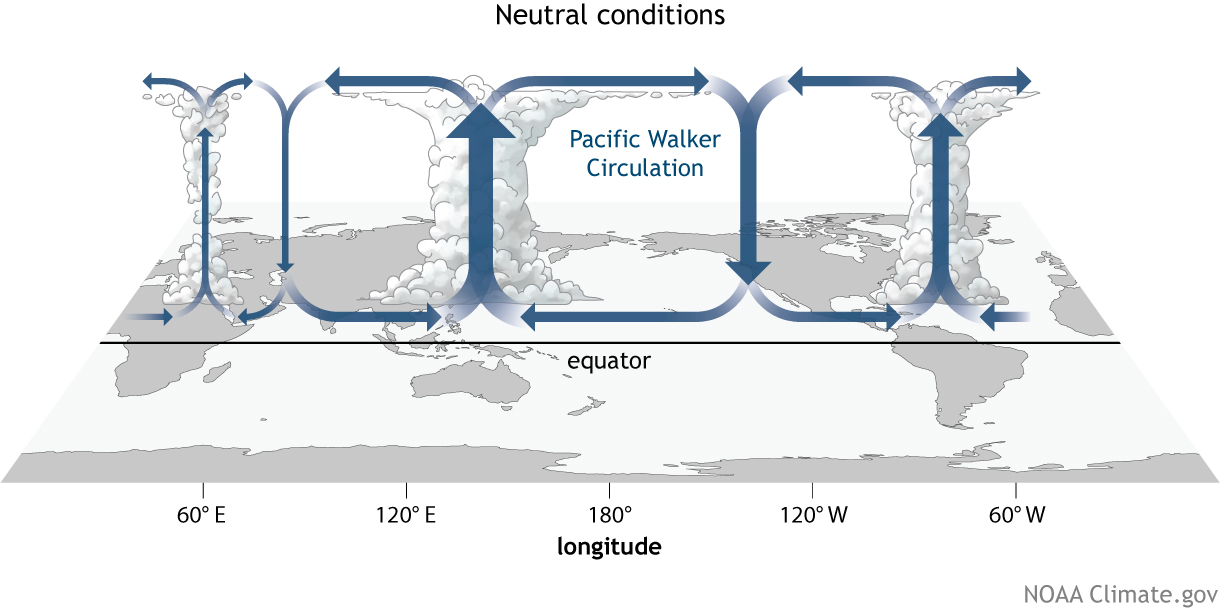
\includegraphics[width=\linewidth]{figures/Walker_Neutral_large.jpg}
\caption[The Walker circulation]{A schematic of the Walker circulation, depicting the mean zonal and vertical circulations, under neutral conditions of El Niño-Southern Oscillation. Schematic originally from: \url{www.climate.gov/}. }
\label{fig:walker_schematic}
\end{figure}
 
 
The Hadley cell is the meridional overturning circulation that arises from the differential heating between the tropics and the midlatitudes. This overturning cell is characterized by ascending motions in the tropics and descending motions in the subtropics and acts to transport heat poleward from the equator \citep{lorenz1967}.  The ascending section of the Hadley circulation migrates meridionally with the seasonal cycle, the winter and summer cells interact with each other but also with the midlatitudes through eddy momentum fluxes \citep{bordoni2008monsoons}. 
The Hadley cell is not zonally symmetric; the boreal summer Hadley cell, for instance,  is primarily a result of ascent in the Indian Ocean and the West Pacific regions with a minor contribution from ascending motions in Central and North America \citep{hoskins2020}. 

\added{In turn, zonal circulations also exist in the tropical atmosphere and the most prominent example is the Walker circulation. }
The Walker circulation is the zonal overturning circulation that is found in the equatorial Pacific Ocean, illustrated in Figure \ref{fig:walker_schematic} and characterized by ascending motion over the West Pacific and descending motions over the East Pacific \citep{walker1924,bjerknes1969,gill1980}. The dynamic and thermodynamic effects of the location and strength of convection associated with the Walker circulation have strong impacts across the tropical and extra-tropical atmosphere, known as teleconnections \citep{cai2019pantropical}.

\added{Another relevant aspect of the tropical circulation is the Intertropical Convergence Zone (ITCZ), which is a tropical band of convective clouds and precipitation that migrates meridionally with the seasons, characterized by a strong convergent flow at low levels and a strong divergent flow at upper levels \citep{schneider2014}. The ITCZ is intertwined with the Hadley cell as the position of the ITCZ is collocated with the ascending branch of the Hadley cell \citep{donohoe2013,hartmann2015}}, and is arguably one of the most relevant features of tropical climate due to the strong influence of convective activity in the ITCZ over the low- and upper-level circulation, tropospheric latent heating due to deep moist convection, as well as the fact that the largest precipitation rates in the tropics are found in the ITCZ.

The position and strength of the ITCZ results from the inter-hemispheric energy and momentum balances so that the ITCZ is predominantly north of the equator because of the inter-hemispheric temperature contrast  \citep{donohoe2013,bischoff2016}. 
\added{Over regional scales, the seasonal migration of the ITCZ follows closely the seasonal cycle of SSTs, which depends on the solar insolation and the coupling between SST gradients, cloud radiative heating and the low-level easterly flow \citep{richter2014equatorial,siongco2015,oueslati2015,harrop2016}.
Variability in the characteristics of the ITCZ can affect relatively remote regions through impacts in the tropical convective heating, a modulation of the wave-train propagation and of the strength and location of mass-flux descent  \citep{neelin2005,neelin2007moist,cai2019pantropical}.}


\begin{figure}[t!]
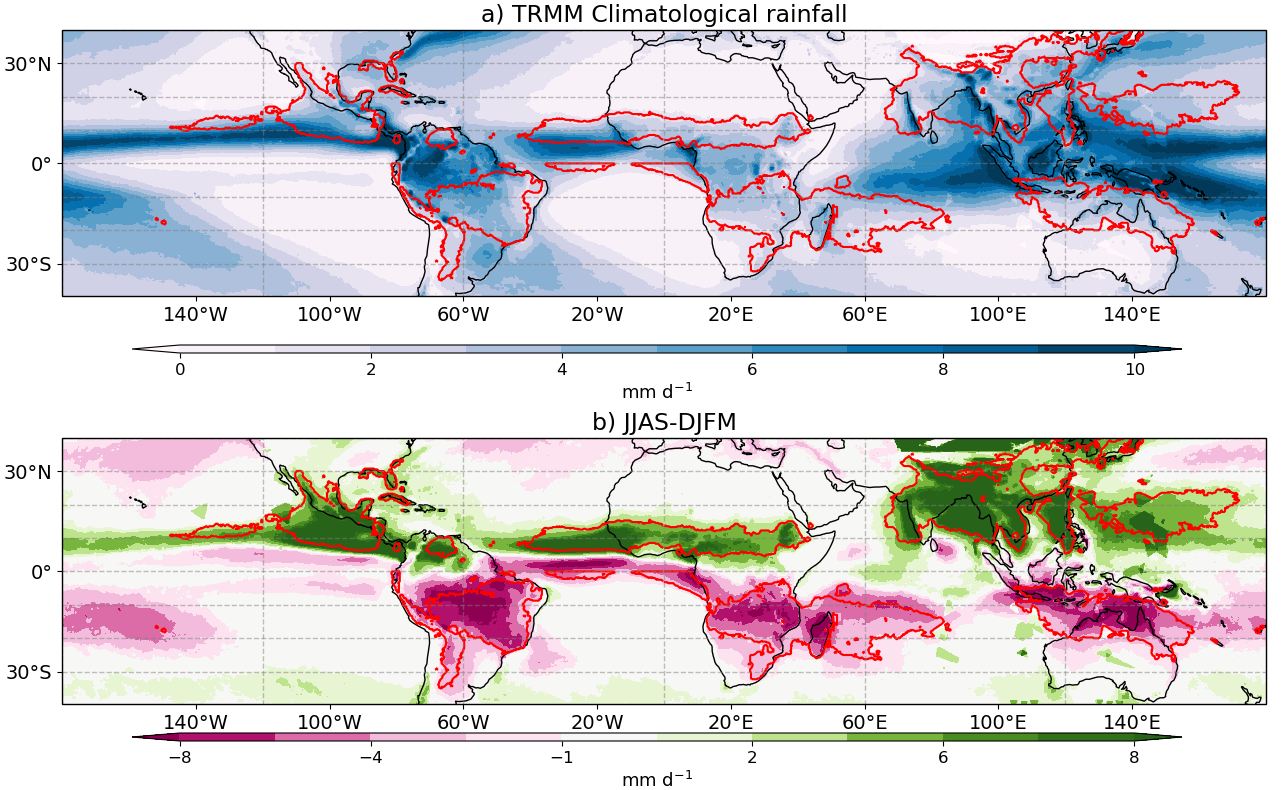
\includegraphics[width=\linewidth]{figures/trmmclima.png}
\caption[The global monsoon rainfall]{a) Climatological mean annual rainfall rates in the tropics using data from the Tropical Rainfall Measurement Mission (TRMM) dataset (1999-2018). b) The mean rainfall rate difference between boreal summer (JJAS) and austral summer (DJFM). The red contours highlight the regions where the mean summer rainfall amount accounts for more than 55\% of the mean total annual rainfall accumulation. }
\label{fig:monsoon}
\end{figure}

In spite of the global impact of the ITCZ and tropical circulations, one of the phenomena of tropical climate that first generated research interest is the monsoon \citep{halley}. The word \textit{monsoon} stems from the Arabic word for \textit{season} and this definition illustrates the very first conceptions of a monsoon. 
The first widely accepted view of a monsoon suggested that it was the result of a large-scale land-sea breeze associated with the differential warming of the land and the ocean that force a seasonal reversal of the low-level winds bringing seasonal rainfall to a region \citep{halley}. 

The traditional definition of the monsoon as a land-sea breeze has several shortcomings. Firstly, several mid-latitude regions would fit a monsoon definition based solely on a seasonal reversal of the wind \citep{gadgil2018}, and secondly, regions that are now recognized as a region with a monsoon climate, e.g. in South America, do not show a seasonal reversal of the winds, and the wind flow may just exhibit seasonal changes in direction and strength \citep{vera2006}. For these reasons, the land-sea breeze view of monsoons has recently been replaced by three alternative conceptions, an ITCZ-monsoon framework, a convective quasi-equilibrium interpretation and a moist static energy (MSE) zonal-mean energetic interpretation \citep{biasutti2018global,hill2019,geen2020}. 



The first framework  explains monsoons as a poleward extension of the ITCZ into land  generalizing all monsoons as an expression of global tropical convergence resulting from the energy balance \citep{chao2001origin,gadgil2018}. This interpretation has led to the concept of \textit{the global monsoon}, a term that encompasses all the regions in the tropics that exhibit a strong seasonality in precipitation \citep{zhou2016,gadgil2018}. 
In practice, the global monsoon refers to those regions of the planet where more than 70\% of the total annual rainfall is observed during the local summer season, therefore, the concept of a global monsoon recognises the seasonality of precipitation as the key feature to diagnose a monsoon \citep{zhou2016,wang2017}.

Figure \ref{fig:monsoon} shows the global monsoon as depicted by the TRMM dataset. By this definition, the majority of the regions over land between 5 and 10 degrees away from the equator are part of the global monsoon.
A regional monsoon, such as the Indian Monsoon, is then a subset of the global monsoon with unique regional characteristics that shape this monsoon differently to other regional monsoons in terms of the seasonality, the strength and the dynamics. 
The American Monsoon System is then the regional monsoon that is located in the subtropics of North and South America. 


\cite{bordoni2008monsoons} provide an alternative conceptual view of monsoons, describing the characteristic rapid onset of a monsoon as a regime transition of the Hadley cell from an eddy momentum -driven circulation, which resembles a canonical ITCZ regime, to a thermally direct circulation which resembles a monsoon-like circulation. The zonal mean MSE meridional gradient drives the ITCZ location and determines the strength of the overturning circulation by modulating the ventilation from the midlatitudes that bring cooler and drier air in a feedback mechanism \citep{geen2020}. Even though \cite{bordoni2008monsoons} propose an axisymmetric framework, their predictions were broadly consistent with the Asian monsoon circulation. 


Convective quasi-equilibrium (CQE) is a theory for moist convection where convection sets the vertical temperature and moisture profiles to a convectively neutral state, thereby setting the free tropospheric temperature \citep{neelin2007moist}. For a monsoonal circulation, this theory emphasizes the coupling of convection and dynamics predicting that the sub-cloud layer equivalent potential temperature maxima must be collocated with the free tropospheric saturation equivalent potential temperature \citep{nie2010observational,geen2020}. The rapid onset of the Asian monsoon is associated with the boundary layer moist entropy distribution, in agreement with predictions of CQE \citep{nie2010observational,boos2015review,ma2019}.

Several studies examine the monsoon as a large-scale phenomenon through an axi-symmetric framework that assumes zonal symmetry investigated through global energetic diagnostics \citep[e.g.][]{faulk2017effects,geen2019,byrne2020}. The zonal-mean framework is common to the Hadley cell interpretation of monsoons \citep{bordoni2008monsoons}, as well as the ITCZ-monsoon theory. %This framework is very much in line with the global monsoon concept, that implies a zonally symmetric circulation driven by global energetic balance. 
However, regional monsoons are shaped by the asymmetries imposed by the orography, the characteristics of the surrounding ocean basins, land-sea contrasts and also the role of vegetation-hydrology coupling \citep{wang2017,pascale2019}. 
The importance of zonal asymmetries has raised multiple issues with large-scale so-called monsoon dynamics theories, as several predictions of these theories are not consistent with observations of regional monsoons \citep[e.g.][]{nie2010observational,smyth2018simulated,biasutti2018global,pascale2019}. 


%The MSE budget and methodology are detailed in section \ref{sq:msemethod} but a broad description of the method and summary of results arising from the MSE budget applied to the monsoon phenomena is given below.
 The MSE budget framework suffers both from theoretical and practical shortcomings. One practical shortcoming is that the calculation of the budget terms post hoc in reanalysis or models results in very large residuals \citep{hill2019}, so these frameworks work best when the calculations of the budget terms are integrated online at each time-step \citep[e.g.][]{ma2019}.
Another shortcoming is that the surface fluxes over land, e.g., in the Sonoran and Saharan deserts and the deep Amazon make the estimations of the roles of hydrology-vegetation feedbacks and their potential contributions to the MSE budget in observations very difficult to assess \citep{boos2016,pascale2019}. The use of simpler moisture budgets has proven useful in a regional context to investigate the sources of moisture for monsoons in current  \citep{ordonez2019,martinez2019} and future climates \citep{smyth2020}, but this budget is mostly a tool and not a coherent theory for the dynamics of monsoons.

Recent reviews acknowledge that all these frameworks have significant shortcomings when applied to regional monsoons \citep{biasutti2018global,hill2019,geen2020}. These reviews conclude that a framework that reconciles the global energetic perspective with the characteristics of regional monsoons would be crucially important and very useful, but as several authors point out \citep[e.g.][]{biasutti2018global,hill2019}, also very hard to formulate. \added{There is no detailed physical description of the global monsoon system with a single theoretical formulation that can explain the observed features of all the regional monsoons.}



 
The Hadley cell interpretation of monsoons has significant shortcomings to depict some regional monsoons, particularly those that are not the Asian monsoon as the overturning circulation in the South Asian monsoon is strong enough to be represented by a clear thermally direct regime.
However, this energetic framework assumes no zonal transport of energy, which minimizes the role of orography and land-sea interaction \citep{biasutti2018global}, which may explain why the North American monsoon does not exhibit the circulation described by \cite{bordoni2008monsoons}.
One might reasonably infer from these results that the timing of the transition in the zonal mean overturning cells would be similar for monsoons at different longitudes but similar latitudes, which is not the case \citep{wang2017}.
 


Furthermore, a monsoon restricted to a small area, such as the North American and African monsoons may not show a clear zonally averaged overturning regime and may be significantly affected by local shallow and deep circulations \citep{zhai2015regime}. For instance, \cite{smyth2018simulated} show that the simulated West African monsoon when forced with different solar forcings exhibits a decoupling between the zonal-mean ITCZ location, the strength of the local Hadley cell and the monsoon rainfall, in opposition to the predictions of this framework \citep{bordoni2008monsoons}.


In short, despite significant progress in our understanding of the monsoon phenomena at the planetary scale through zonal mean energetic frameworks, there is an important gap between large-scale theories of monsoon dynamics and the observed regional monsoons. 
The next section presents a summary of the North and South American monsoon literature, which explains the characteristics of these monsoons through the effect of regional features and dynamics, seemingly detached from the literature in this section.

\section{The American Monsoon System}\label{sq:bk_ams}

\begin{figure}[t!]
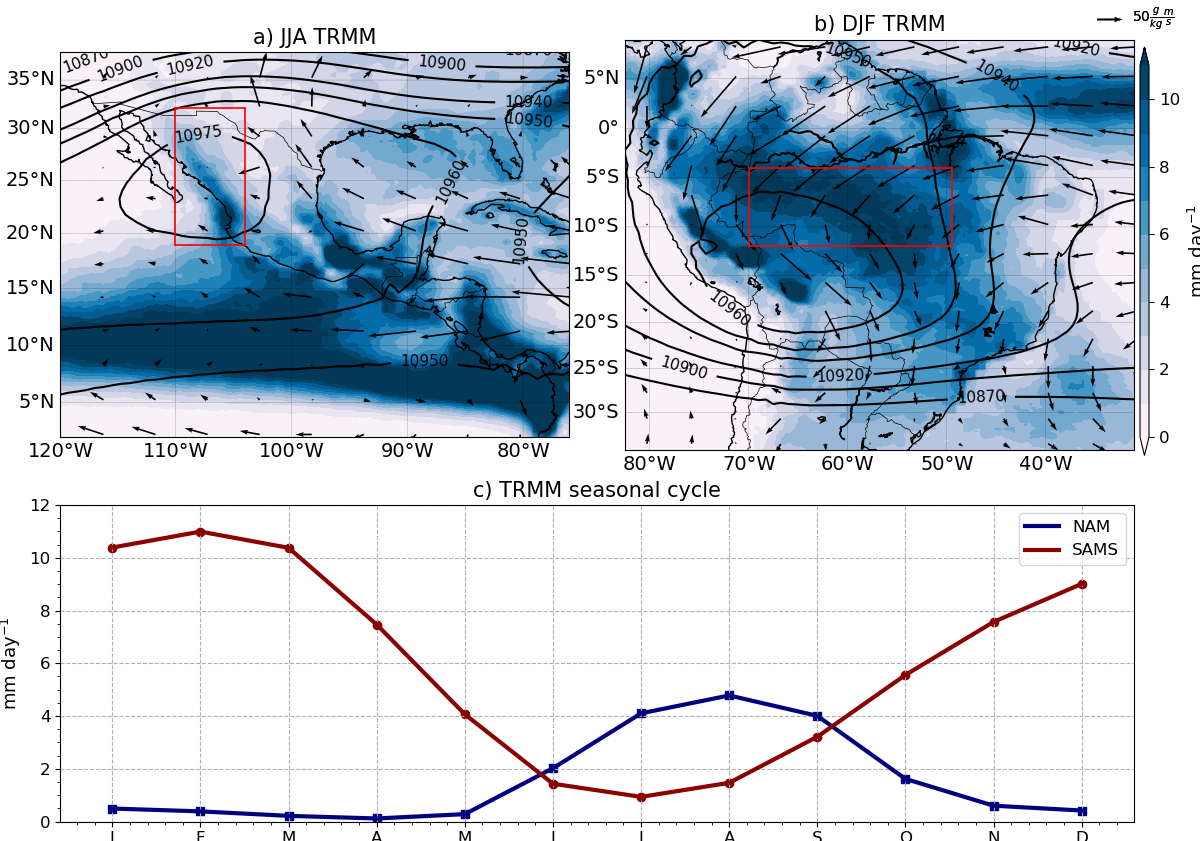
\includegraphics[width=\linewidth]{figures/amsclim.png}
\caption[The American monsoon system climatology]{ Climatological mean a) boreal and b) austral summer rainfall (shading), 850 hPa moisture flux (vectors) and geopotential height at 250 hPa (contours) in a) southern North America and b) South America. c) Monthly-mean seasonal march of precipitation in the TRMM dataset for two area-averaged time-series, the North American Monsoon (NAM) and the South American Monsoon System (SAMS) shown in the red rectangles in a-b). }
\label{fig:americanmonsoon}
\end{figure}

The American Monsoon System (AMS) is the main source of rainfall for tropical Latin America and is typically subdivided into the North and South American monsoon systems \citep{vera2006}. 
Although the spatial definition of the AMS is quite varied amongst studies, a general consensus is that the North American Monsoon is found in south-western North America (Figure \ref{fig:americanmonsoon}a) extending north from central-west Mexico into the southwestern United States and the South American Monsoon is centred in the deep Amazon south to the river mouth (Figure \ref{fig:americanmonsoon}b) but southeastern Brazil  \citep{adams1997,stensrud1997,vera2006}.


 The seasonal cycle of rainfall in the North American Monsoon is characterised by a wet July-August-September season and significantly drier conditions during the rest of the year \citep{adams1997} (Figure \ref{fig:americanmonsoon}c).
Three temporal stages describe the evolution of the North American Monsoon \citep{adams1997,geil2013}.
First, the onset stage (May-June) starts with a strong surface warming that leads to very high temperatures in the desert region.
Simultaneously, the subtropical jet weakens and migrates north decreasing the frequency of mid-latitude disturbances in the monsoon region \citep{douglas1993,turrent2009}.
These factors combine to develop a low-level thermal surface low pressure linked with an upper-level anticyclone and  moisture influx from the nearby Gulf of California and easternmost Pacific Ocean \citep{douglas1993,geil2013}.

Maturity (July-August) is the peak period of monsoon rainfall characterised by sustained deep convection \citep{barlow1998} and significant increases in low and mid-level moisture flux convergence and mid-level latent heating \citep{adams1997,cook2013}. The latent heating caused by deep convection can be diagnosed in the upper-level geopotential height (Figure \ref{fig:americanmonsoon}a) in the form of an anticyclone centred on the monsoon region. 
The moisture flux convergence decreases in August, after which precipitation recycling \citep{dominguez2008} plays an important role in keeping deep convection active until September.
 Decay (September-October) is the last stage of the monsoon, in many ways opposite to the onset stage, as is characterised by the equatorward migration of the subtropical jet \citep{higgins1997,geil2013}, evaporation in the nearby basins decreases and deep convection in the monsoon region disappears \citep{douglas1993}.

 The origin of moisture at low and mid-levels in the monsoon region has been a matter of debate \citep{adams1997,barlow1998,vera2006,ordonez2019}, with 
several studies suggesting that the main source of moisture for the North American Monsoon is the East Pacific Ocean and, to second order, mid-level moisture advected from the Gulf of California \citep[e.g.][]{adams1997,stensrud1997,vera2006,turrent2009,ordonez2019}.
\added{However, a more puzzling aspect is how moisture is exactly advected and organized specifically on the western coast of northern Mexico. Orography seems to be the dominant fact as the Sierra Madre Occidental (SMO) found in the core NAMS region is a key feature of this monsoon.} 

\added{Early studies suggest that the role of the SMO is to channel moisture from the East Pacific and Gulf of California \citep{seastrand2015} or in a mountain-sea breeze mechanism operating with the diurnal cycle of the low-level winds \citep{nesbitt2008diurnal}. However, \cite{boos2021} provides an alternative hypothesis for the role of the SMO in the organization of the monsoon in southwestern North America. Their results suggest that the role of the SMO is to deflect the subtropical jet and produce an eastward upward flow that organizes convection in a confined region with relative high surface moist static energy.}
 

The South American Monsoon System (SAMS) is a primary source of precipitation for South America, especially in the Amazon region \citep{gan2004,vera2006,jones2013}.
During austral summer (DJF), monsoon rainfall accounts for over 60\% of the total annual precipitation in the Amazon \citep{gan2004,marengo2012}, whereas
austral winter rainfall accounts for less than 5\% of the total annual rainfall \citep{vera2006}.
In the central Amazon, convective precipitation is observed from early October but the main rainy season extends from December to April \citep{machado2004,adams2013}, whereas convection in southeastern Brazil and Paraguay starts in November and peaks in January and February \citep{marengo2001,nieto2011}. A surface heat low appears in Bolivia in early austral summer, known as El Chaco Low, as a result of strong warming in austral spring \citep{marengo2012,sulca2018}.
 Simultaneously, an upper-level anti-cyclone (Fig. \ref{fig:americanmonsoon}b), known as the Bolivian High, develops in the same region as a signature of strong deep convection and latent heating \citep{marengo2001,vera2006}.


\added{The South American Low-Level Jet (SALLJ) and the South Atlantic Convergence Zone (SACZ) are two primary climatic features of the SAMS \citep{vera2006,marengo2012,jones2019recent}.
The SACZ is observed as a nortwest-southeast oriented band of convection  \citep{carvalho2004,nobre2012coupled,jorgetti2014,zilli2019} that is more frequently active during austral summer in association with the onset of the SAMS \citep{marengo2012,perez2021}.    }

\added{The coherent band of organized convection in the SACZ forms from the convergence of moisture emanating from the South Atlantic Subtropical High and from the northerly flow from the Amazon \citep{marengo2012,zilli2019}. Moreover, mid-latitude disturbances or wave-trains are key for the establishment  and variability of the SACZ \citep{carvalho2004,nieto2013aqua,van2015dynamical,zilli2021rossby}. Variability of the SACZ diagnosed as shifts to the position and strength of the band of convection are intertwined with the continental-scale moisture transport and precipitation in south eastern Brazil and central South America \citep{mo2001pacific,jorgetti2014,perez2021}.}

\added{The low-level wind circulation imports moisture from the Atlantic Ocean, once the flow has crossed through the Amazon, the low-level winds are steered by the Andes cordillera into the SALLJ \citep{geen2019,jones2019recent}. The variability of the SALLJ can modulate active and break phases of the monsoon as well as active days of the SACZ, through the modulation of the moisture transport across the continent \citep[e.g.][]{liebmann2011,grimm2011,jones2019recent}. In short, the SACZ and the SALLJ are prominent features of the mean SAMS but their variability also modulates the SAMS precipitation on multiple temporal timescales \citep[e.g.][]{marengo2012,junquas2012summer,perez2021}. }

\added{ South American orography, which features the long Andes cordillera, has long been investigated for its role in the dynamics of the SAMS \citep[e.g.][]{rodwell2001subtropical,campetella2002influence,insel2010influence,
saurral2015links,junquas2016influence}. Evidence shows that the Andes cordillera deflects the low-level wind flow from the equatorial Atlantic southward mechanically forcing the SALLJ \citep{campetella2002influence,insel2010influence} and thereby contributing to the tropical-to-subtropical moisture transport. 
The Andes cordillera also blocks the westerly winds from the Pacific Ocean which would ventilate low-level moisture in South America \citep{insel2010influence} and the existence of the cordillera is key to the formation and location of the SACZ \citep{junquas2016influence}.
 }


\added{The global monsoon theories discussed in the previous section struggle to accurately depict several aspects of the NAMS and the SAMS.
For example, the North and South American Monsoons depart from CQE, as precipitation does not follow the maxima in sub-cloud equivalent potential temperature \citep{nie2010observational,geen2020}. The role of orography and soil-atmosphere interactions may be playing a big part in both the SMO and the Amazon to decouple the sub-cloud MSE and the free troposphere \citep[see e.g.][]{boos2021}.
One alternative hypothesis is that ventilation of low moist entropy air from the midlatitudes is responsible for this decoupling of the boundary layer and the free troposphere in the American monsoons \citep{boos2015review}.
Similarly, the meridional circulations associated with these monsoons do not fit the framework of \cite{bordoni2008monsoons}, which suggests an alignment of the maximum ascent with the maximum surface MSE, which is not observed in either monsoon of the AMS. 
As such, existing monsoon theories either do not fit the observed AMS, or need to be tailored to explain only one of these monsoons.  }


%The SAMS and NAM did not fit the tradditional view of monsoons as the seasonal reversal of the winds was not as strong and clear as for other monsoons such as the Indian monsoon \citep{}. However, there is seasonal contrast in the zonal winds in both the NAM and SAMs as composite DJF-JJA wind differences suggest. 
%Furthermore, the NAM lower-level temperature structure departs from the quasi-equilibrium framework. A monsoon, can be described, through quasi-equilibrium arguments, \citep{}. %structures

\section{A review of the physical mechanisms for the Midsummer drought}\label{sq:litmsd}


The characteristics of the seasonal cycle of precipitation in northwestern Central America, the Caribbean and southern Mexico fit the definition of a monsoon climate \citep{wang2017} with a clear separation of the wet and dry seasons.
However, this region shows a unique climatological precipitation feature. After monsoon onset, rainfall decreases considerably around midsummer; this decrease is followed by a secondary increase in precipitation in the late summer \citep{mosino1966}, and for this reason this feature of the seasonal cycle is most commonly referred to in the literature as the Midsummer drought (MSD) \citep{magana1999}.    \added{ Although the MSD regions sometimes features in AMS studies \citep[see e.g.][]{pascale2019}, and is technically part of North America by some definitions, this region is not considered to be part of the North American monsoon.}


The intraseasonal variations of precipitation associated with the MSD have been known for centuries and have shaped agricultural practices in the region. 
For example,  ancient Mayan texts suggest that agricultural rituals associated with the plea for rain-bearing clouds to the gods were significantly more frequent during the drier MSD period \citep{jobbova2018ritual}. In current days, the MSD is well known by local farmers who refer to the drier midsummer period as `El Veranillo' in Central America and `can\' icula' in southern Mexico because the drier period  coincides with the Canis Major constellation appearing in the sky \citep{dilley1996}.

% so that the MSD variations have shaped agricultural practices in the region for centuries.
%
% Save paragraph for onset method! 
%Farmers in Central America who are subject to climatic stress due to droughts, have already perceived and adapted to changes in the characteristics of the rainy season, such as the timing and strength of the midsummer drought \citep{hellin2017,de2018,harvey2018}, but it is unclear whether these perceived changes are a real trend in the observations \citep{anderson2019multiscale}. 

The two peak structure of the MSD has been diagnosed in the observed climatological precipitation of several regions of Mexico, El Salvador, Belize, Guatemala, Costa Rica and Cuba \citep[e.g.][]{mosino1966,magana1999,duranquesada2017,perdigon2018,martinez2019}.
However, notable differences in the seasonal cycle of precipitation have been found between mainland Central America and the Caribbean islands. The so-called first peak of precipitation occurs in June and the second peak in September in northern Central America whereas the two peaks are observed in May and October in the Caribbean.

\begin{figure}[t!]
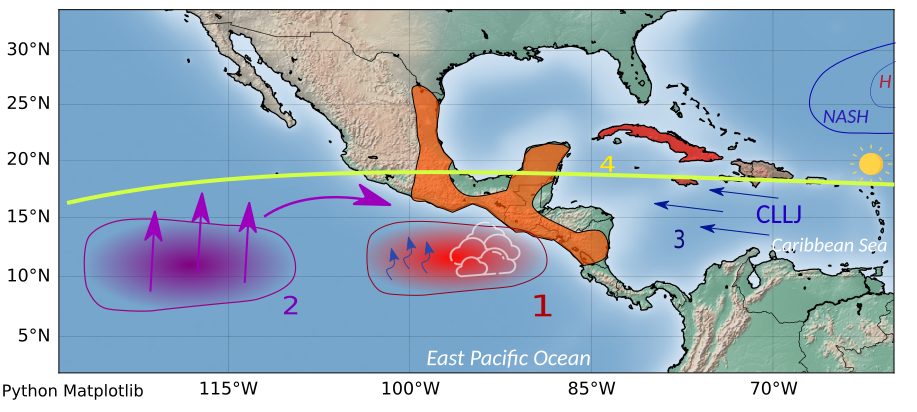
\includegraphics[width=\linewidth]{figures/back_msd_diag.png}
\caption[Mechanisms of the Midsummer drought]{A schematic of the Intra Americas Seas region, depicting the four main mechanisms associated with the Midsummer drought in Mesoamerica (orange) and the Caribbean region (red). (1) The radiative-convective feedback mechanism associated with a double peak in East Pacific SSTs proposed by \cite{magana1999}. (2) The ascending region west of the continent produces an anomalous descending motion over the continent through a direct circulation, argues \cite{herrera2015}. (3) The Caribbean Low-Level Jet (CLLJ) modulates the moisture transport for all the region, with several studies supporting the hypothesis that seasonal cycle in the CLLJ is the main mechanism for seasonal fluctuations in rainfall \citep{duranquesada2017,martinez2019}. (4) The double-crossing of the solar declination angle, proposed by \cite{karnauskas2013}, suggests that each peak of precipitation is associated with peaks in the total shortwave radiation reaching the surface. \added{Note that the Mesoamerican MSD is not part of the North American monsoon \citep{adams1997}.}  }
\label{fig:msd_schematic}
\end{figure}

%The mechanisms that cause the MSD have been debated since the first observational descriptions of the phenomenon \citep[e.g.][]{mosino1966}, as studies that aimed to explain the physical mechanisms MSD have not yet reached a consensus.
 Despite extensive research to understand the physical mechanisms associated with the MSD   \citep[e.g.][]{magana1999,giannini2000,gamble2008,herrera2015,maldonado2017,straffon2019}, debate remains over which is the leading-order mechanism that causes rainfall to decrease at midsummer and increase again at the end of the summer.  % why rainfall increases again at the end of the summer, the end of the MSD, and why this happens at this time of the year. 
%Dynamical or thermodynamical mechanisms have been put forth and different roles have been proposed for the Atlantic and the East Pacific Oceans \citep[e.g.][]{magana2005,gamble2008,herrera2015}. 
Fundamental questions remain unclear such  as whether the MSD is caused by two precipitation enhancing mechanisms \citep{karnauskas2013} or a mechanism that inhibits rainfall at midsummer \citep{duranquesada2017}. 
Furthermore, the association between the MSD in Central America and the Caribbean is still disputed \citep{gamble2008}, as most studies suggest that the two regimes are unrelated and therefore two different explanations are required to account for the two MSDs in these regions. 
Figure \ref{fig:msd_schematic} summarises the four main mechanisms that will be addressed in this section and this thesis. 

%Any complete theory or conceptual model must account for the following characteristics of the seasonal cycle. First, the theory must explain the timing and strength of the first peak of rainfall. Second, the timing and strength of the MSD, i.e., what causes rainfall to decrease at midsummer. Finally, the theory must explain the timing and mechanism driving the second increase in precipitation after the midsummer. %The lack of a clear understanding of the processes that modulate the MSD makes climate change projections uncertain. 

One of the first hypotheses to account for the bi-modal distribution of rainfall was proposed by \cite{hastenrath1967} who argue that a double-crossing of the ITCZ can explain the MSD so that the first peak of precipitation is associated with early summer northward crossing of the ITCZ and the second peak the return or southward displacement of the ITCZ during late summer.
However, this theory fails to explain the MSD signal seen at latitudes as high as 29$^\circ$N \citep{perdigon2018,zhao2020}, which is further north than the northernmost extension of the ITCZ \citep{schneider2014}, and the ITCZ does not cross twice so far from the equator. % \citep{magana1999,magana2005}.

\cite{magana1999} and \cite{magana2005} proposed a mechanism driven by radiative-convective feedbacks between the East Pacific (EP) sea-surface temperatures (SSTs) and deep tropical convective clouds (mechanism 1 in Figure \ref{fig:msd_schematic}). The coupling between the height and strength of convection, the incoming shortwave radiation and the SSTs are the key features of their framework. %Convection feedbacks with SSTs evaporation and
%moisture flux into the MSD region. 
The EP SSTs peak in May triggering large evaporative fluxes and deep convection in the EP ITCZ and the western coast of Central America.
The high convective clouds produce a radiative cooling effect at the surface due to a decreased incoming shortwave radiation associated with the reflectance of shortwave radiation by clouds.
This cooling  decreases SSTs and deep convective activity and thus accounts for the decrease of rainfall during midsummer.
The second peak in September is driven by an opposite mechanism, i.e., the decreased frequency of deep convective clouds during the MSD period in July and August reduces the cooling effect of the anvil clouds and increase the incoming shortwave radiation at the surface, SSTs and surface fluxes, all of which leads to an increase in precipitation during late August and September \citep{magana1999}.


%have been linked to several sources of seasonal variability,
%but debate is far from uncontroversial as to which is the principal mechanism to account for the MSD.
A large number of studies, in contrast, propose that the seasonal evolution of the North Atlantic Subtropical High (NASH) is the leading mechanism for the MSD \citep[e.g.][]{mapes2005,small2007,gamble2008,curtis2008,munoz2008,martinez2019,corrales2020}. The NASH is the subtropical anticyclone in the North Atlantic Ocean that migrates southwest during early boreal summer. The expansion and intensification of the NASH in boreal summer, according to these studies, strengthens the low-level trade winds, controlling the seasonal cycle of a low-level jet found in the core of the Caribbean Sea known as the Caribbean Low-Level Jet (CLLJ). 

The CLLJ is a key regional feature of the climate of the Caribbean and the Intra-Americas Sea  because the strength and direction of the flow in the Caribbean controls the underlying Caribbean SSTs and the regional moisture transport \citep{giannini2000,mestas2007,martinez2019,garcia2020sub}. 
 However, studies disagree on the specific roles that the CLLJ and the NASH play to modulate seasonal cycle of precipitation over the Mesoamerican region. 
 For example, some studies \citep[e.g.][]{giannini2000,mestas2007,gamble2008} suggest that  the expansion of the western flank of the NASH strengthens the CLLJ which cools the SSTs, through the effect of wind stress and mixed-layer mixing.
The cooling of SSTs diminishes evaporation and therefore low-level moisture which ultimately leads to less precipitation. In contrast, other studies propose that the seasonal cycle of the CLLJ (mechanism 3 in Figure \ref{fig:msd_schematic}) modulates seasonal variations of precipitation by modulating the regional moisture transport  \citep{small2007,munoz2008,herrera2015,duranquesada2017,martinez2019}. In this second hypothesis, the changes to the intensity of CLLJ influenced by the NASH modify the convergence and divergence patterns in the Intra-Americas Sea. In other words, the midsummer strengthening of the CLLJ increases moisture divergence, drying the atmospheric column over the Caribbean. 


%GCM literature needed.
 
    
%The strength of the easterlies crossing from the Caribbean Sea to the EP Ocean has been argued to modulate ascending and descending motions all across the Intra-Americas Seas region through the  effects of vertical wind shear and moisture divergence  \citep{herrera2015,corrales2020,zhao2020}. Moisture budgets over the Caribbean have diagnosed that changes to the regional and temporal distribution of moisture \citep{duranquesada2017,martinez2019,martinez2020} can influence the intra-seasonal and inter-annual variability of precipitation. % can be explained by the variability of the easterly wind flow in the CLLJ and the EP Ocean \citep{herrera2015,martinez2019,zhao2020}. 


%The strength of the flow crossing  between the EP Ocean and the Caribbean Sea has been argued to be a a function of the SST gradient across the basins, at least on interannual time-scales \citep{martinez2020}. This is particularly relevant as the Pacific Ocean is projected to warm more than the Caribbean Sea in future decades, which could change the SST gradient, strengthen the CLLJ and shift the regional precipitation patterns \citep{corrales2020}.
    
 \cite{herrera2015} show that during the drier months in Central America in the Midsummer, convective activity west of the central American continent gets stronger with heavier precipitation (mechanism 2 in Figure \ref{fig:msd_schematic}).  Their evidence suggests that the gap flow that originated from the CLLJ in the Caribbean Sea controls the location of ascending and descending motions, and the MSD may be explained by the seasonal variations of the coupling of the low-level wind flow with the underlying EP SSTs.
\cite{herrera2015} further argued that the exit region of the CLLJ is located to the east of the region of the strongest MSD signal, which suggests that the moisture divergence effect over the central American MSD is minimal. 

A different mechanism, proposed by \cite{karnauskas2013}, argues that the biannual crossing of the solar declination angle can control precipitation and explains the bimodal characteristics of the seasonal cycle (mechanism 4 in Figure \ref{fig:msd_schematic}). In this mechanism, the MSD is driven by two precipitation enhancing periods that are separated by a relatively normal, and drier, period. This theory differs from those previously discussed which explained the MSD through mechanisms that inhibit convective activity in the midsummer whereas \cite{karnauskas2013} argues that the solar declination angle that crosses twice through Central America, once during June and a second time during September, increases convective activity during each crossing. 

The variations of incoming shortwave radiation associated with the declination angle modulate the SSTs, surface fluxes and therefore convective activity. In other words, the first crossing of the solar declination angle increases the incoming shortwave radiation which increases the SSTs, evaporation and leads to a peak of precipitation, i.e., the first peak. After the shortwave radiation is reduced the MSD period appears. The second crossing of the solar declination angle, similarly, explains the second peak as the second increase in incoming shortwave radiation drives an increase in deep convection.% than during the MSD. 

Other mechanisms have been proposed arguing that the MSD is a result of vertical wind shear affecting convective instability or the Saharan dust controlling  the microphysics of clouds \citep{angeles2010origins}.
For instance, \cite{perdigon2019} also finds a link between the frequency and spatial distribution of the first peak rainfall rates and the Madden-Julian Oscillation (MJO). 
\added{In short, a plethora of hypotheses exist for the causes of the MSD, however, a key aspect of the climate of the AMS, is the effect of ENSO, which is the following section.}
 
\section{El Niño Southern Oscillation: impacts on the American monsoon system}
\label{sub:lit_enso}



 El Niño-Southern Oscillation (ENSO) coupled ocean-atmosphere phenomenon in the equatorial Pacific Ocean that is profoundly important for the global climate system, which is why ENSO is commonly known as the leading mode of interannual variability. 
 The term \textit{'El Niño'} was coined by Spanish colonizers when they learnt from Peruvian fishermen that the SSTs in the easternmost Pacific Ocean increased notably in some years around December time. 
 Later on, sir Gilbert \cite{walker1924} coined the term \textit{Southern Oscillation} to describe the synchronous changes to the sea-level pressure of the Indo-Pacific region and South America.% and further research \citep[e.g.][]{troup1965} would highlight that these remote changes in pressure were driven by the east-west pressure gradient in the equatorial Pacific. 
% For religious reasons, the colonizers termed the SST increase as Christ Child -- \textit{El Niño}. 
 %The effect teleconnections can be felt in the tropics through changes in the tropical overturning circulation but also impacting extratropical circulations and thus ENSO impacts extend to most regions on the planet.
 
 
 
  
 % \cite{walker1924} and \cite{walker1932} are the first analyses of synchronous effects of the tropical circulation over local precipitation, temperature and pressure. 
  
    The changes in the pressure field associated with the Southern Oscillation are now part of what is known as the Walker circulation, which intertwines the dynamics of the zonal circulation in the East Pacific with the SSTs over the underlying ocean. ENSO is then characterized as a coupled phenomenon composed of an oceanic part, \textit{El Niño}, and an atmospheric component associated with the zonal circulation but best characterized by changes to the surface pressure field, i.e., the Southern Oscillation. 
  
  
% The SO changes are intertwined with changes to the Walker circulation as the surface pressure variations affect the strength of low-level trade winds, which are a big component of the Walker circulation. In other words,   ENSO is the coupled ocean-atmosphere oscillation of the equatorial Pacific sea-surface temperatures (SSTs) and the atmospheric pressure and wind fields, particularly those associated with the Walker circulation\citep{wang2004}. %; these variations in the SO are typically described as with the Walker circulation. %changes and the Southern Oscillation (SO) is associated with changes in the zonal gradient of MSLP. Combined, El Niño and the SO compose the ENSO phenomenon.
  
\begin{figure}[t!]
\centering
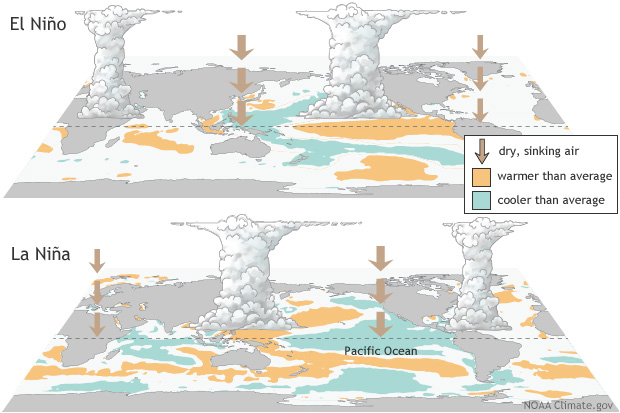
\includegraphics[width=\linewidth]{figures/ENSO}
\caption[El Niño Southern Oscillation and the Walker circulation]{Schematic of the positive (upper) and negative (lower) phases of ENSO. Regions with tall clouds indicate more ascent and convection than normal whereas brown arrrows indicate dry descending air. Obtained from the National Oceanic and Atmospheric Administration at \url{https://www.climate.gov/enso}. }
\label{fig:enso}
\end{figure}  

 ENSO has several unique features, such as no robust periodicity as events may occur every 2 to 7 years and a seasonal phase-locking that are associated with ENSO events peaking in boreal winter in observations \citep{wang2004}. Even though the underlying physics that cause ENSO and explain the variability in the periodicity of the phenomena is still debated \citep{wang2004,christensen2017}, several aspects are now better understood. 
For example, the impact of ENSO events on the location and strength of deep convection in the equatorial Pacific have been thoroughly described and the teleconnections pathways of ENSO are well characterized \citep{trenberth1997,neelin1998}.

During a neutral state of ENSO, the Walker circulation is found in the climatological state, with ascent and wet conditions in the West Pacific  and descent and drier conditions in the East Pacific. During El Niño the Walker circulation and low-level trade winds weaken which is associated with an eastward shift of deep convection along the equatorial Pacific (Figure \ref{fig:enso}), with convective rainfall becoming more frequent in the central and even eastern Pacific than normal \citep{neelin1998,wang2004}. During La Niña the opposite happens and the Walker circulation strengthens which leads to stronger convection in the West Pacific and stronger ascent on the East Pacific (Figure \ref{fig:enso}). 


In other words, ENSO imposes a strong control on the location and strength of the Walker circulation (Figure \ref{fig:enso}). These changes to the strength and position of the convective regions in the Pacific Ocean can then propagate to other regions of the planet; these far-distant effects are commonly known as \textit{teleconnections}.  
\added{ENSO teleconnections work through various pathways or mechanisms. }
For example, Figure \ref{fig:enso} shows the impact of ENSO over other tropical regions outside of the Pacific through the Walker circulation, as upper-level wind anomalies induce anomalous vertical motions over West Africa \citep{ropelewski1986,ropelewski1987} or South America \citep{sulca2018}.  
  Other mechanisms of ENSO teleconnections include extra-tropical routes which include changes to the position and strength of subtropical jets \citep{fereday2020}, changes to the Pacific and North American circulation patterns \citep{bayr2019} as well as impacts to the North Atlantic via the stratospheric polar vortex \citep{domeisen2019}.
  
 \added{ENSO teleconnections impact the AMS both through the tropical and the extratropical pathways \citep{marengo2012,sulca2018,cai2020}. 
 The extratropical pathway refers to these anomalous Rossby wave-trains caused by tropical convective heating that propagate from the equatorial Pacific to the extratropical Pacific and Atlantic affecting  both  northern and southern hemispheres \citep{hoskins1981steady,jimenez2018tropospheric,fereday2020}. The influence of ENSO on the subtropical jets, or the storm track, can impact boreal winter climate in subtropical North and South America \citep{marengo2012,bayr2019}. }
 
 \added{ These wave-driven anomalies cause differences in the regional sea-level pressure systems and the location of the storm track. For example, ENSO induces changes to the Aleutian Low pressure system and similar SLP anomalies of opposite sign over the North American continent, in a teleconnection pattern that is more commonly referred to as the Pacific-North American (PNA) \citep{deser2010sea,bayr2019,jimenezesteve2020}. A similar teleconnection is observed as wave trains travelling from the South Pacific to the South Atlantic, i.e., the Pacific-South American (PSA) pattern \citep{mo2001pacific,vera2009,cai2020}. Specifically, El Niño events induce a positive phase of the PNA pattern during boreal winter which leads to enhanced precipitation and colder conditions over northern Mexico due to the increased frequency of the intrusion of cold mid-latitude disturbances \citep{magana2003}. }
  
  
  \added{The tropical pathway involves the changes to the location and strength of the Walker circulation explained above, in which anomalous descending and ascending anomalies are found in the Amazon region for El Niño and La Niña years, respectively. 
  Another relevant pathway is the impact of ENSO associated with the PNA pattern, which induces changes to the easterly trade winds in the subtropical Atlantic and subsequent impacts to the ITCZ \citep{hastenrath2006,fereday2020}. For instance, El Niño teleconnections throught the PNA pattern lead to a warming of the northern equatorial Atlantic SSTs and induce a delay in the seasonal migration southwards of the Atlantic ITCZ causing a drying of the northern South America \citep{hastenrath2006,cai2020}. The influence of the northern tropical Atlantic and the delay in the southward shift of the Atlantic ITCZ has been shown to influence not only northeastern Brazil rainfall but also extreme events throughout the SAMS \citep{yoon2010atlantic,andreoli2012seasonal,jimenez2021}.  }
  %{In South America, the effects of ENSO are felt throughout the continent, e.g., by Peruvian fishermen \citep{takahashi2004} or in the Amazon rainforest and the plainlands in South-Eastern South America \citep{grimm2011,marengo2012}.}
 
 
 \added{
  Current research on ENSO teleconnections to South America focuses on the observed non-linearity and non-symmetry of the impacts, which has mainly been attributed to ENSO diversity \citep{tedeschi2015,cai2020,jimenez2021}.
 ENSO diversity refers to the observed feature that the maximum SST anomaly does not always appear in the same region of the Pacific Ocean \citep{ashok2009,dommenget2013}. These differences in the SST patterns are referred to as ENSO \textit{flavours} which can be broadly summarized as two flavours for each phase. The flavours are defined based on the location of the SST anomaly so the most common division is into Central and Eastern Pacific events.  In observations, each type of event is usually also associated with the strength of the event \citep{dommenget2013}, with eastern Pacific events being usually stronger than Central Pacific events. }
  
  \added{ENSO diversity has important implications for global teleconnections;  specifically, precipitation impacts and the occurrence of droughts in the SAMS have been linked to non-linear effects associated with the location of the SST anomalies in the Pacific \citep{rodrigues2011,sulca2018,cai2020,jimenez2021}. 
  \cite{cai2020} provides a recent review on the differences in the impacts that Central and Eastern Pacific (CP and EP) events have on South American precipitation and climate features.
The observed record shows that the teleconnections affecting the Amazon and northeastern Brazil are most pronounced during EP El Niño events and CP La Niña events than the CP El Niño events and EP La Niña events. }

 \added{This recent review also highlights the need for further modelling work to test observation-driven hypothesis, as the observed record is too short to make confident statements about the mechanisms associated with non-linear ENSO teleconnections. Specifically, there are still open questions regarding the effect of other climate variability factors on the teleconnections, particularly for different ENSO flavours, and the role of other ocean basins such as the Indian and Atlantic Oceans in the modulation of ENSO effects \citep{cai2019pantropical}. 
 }
  
  
%A non-linear teleconnection refers to a non-linear scaling between the strength of an ENSO event, typically measured by an SST index, and the magnitude of the response, in most cases precipitation response. %So two observed ENSO events, although very similar in magnitude may show different strengths and even patterns in these teleconnections \citep{}. 






%ENSO has motivated extensive research using GCMs to understand the mechanisms related the origin of ENSO \citep{christensen2017}, the feedbacks and processes that phase-lock the phenomena \citep{neelin1998}, as well as how will ENSO characteristics change in the future \citep{cai2015a,santoso2017}.


 
 
 


%The period of ENSO of 2-7 years \citep{neelin1998,wang2004} was poorly represented in CMIP3 and CMIP5 models \citep{guilyardi2009}, particularly by models that had much stronger power spectrums than the observed.



\section{The QBO and tropical convection}\label{sq:qbolit}

%\begin{figure}
%\centering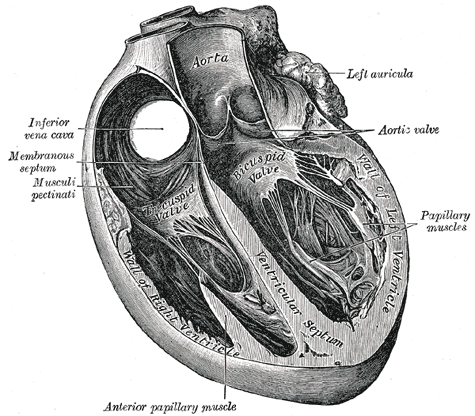
\includegraphics[width=0.7\textwidth]{figures/sample/Gray498.png} 
%\caption[Four-chamber illustration of the human heart.]{Four-chamber illustration of the human heart.  Clockwise from upper-left: right atrium, left atrium, left ventricle, right ventricle.}
%\label{fig:fourchamber}\end{figure}
%The troposphere is the lowermost layer of the atmosphere ranging from the surface up to 10-15 km where the vertical temperature profile is characterized by a decrease of temperature with height so that convective instability plays an important role for vertical motions.
%The layer above the troposphere is called the \textit{stratosphere} where the vertical temperature gradient is reversed and temperatures increase with height so that the atmosphere is stable to upward motions, this layer and spans from . 
%The transition layer in between the troposphere and the stratosphere is referred to as the tropopause, which is a transition region where the vertical temperature gradient reverses and the atmosphere is stable to upward motions. 
%
%%The chemistry and dynamics of the stratosphere are very different from the troposphere both in temporal and spatial scales. The stratosphere is generally drier and well-mixed so that local ultraviolet absorption and infrared radiative loss exert the largest influence over the seasonal cycle of temperature and zonal winds in this layer \citep{andrews1987}.
%%The strength of the inversion layer of the tropopause prevents ascending tropospheric parcels from entering the stratosphere. However, the tropopshere and stratosphere do communicate and exchange momentum and mass through waves, intrusions and radiation. 
%% These exchanges typically include the tropopause. exists between stratosphere and troposphere. 
%
%Stratosphere-troposphere coupling refers to events or processes where the two layers are notably affected by each other so that the temperature or wind flow of the two layers vary together, or \textit{couple}. One prominent example of this coupling is the effect of the stratospheric polar vortices over the zonal flow in the troposphere \citep{thompson2005,domeisen2019}. 
%However, semi-periodic climatic variability in either layer can also have effects over the other layer. The dominant mode of interannual variability in the equatorial stratosphere is such an example and is introduced in the following section. 

% in the  Generally, stratospheric processes are slower and can communicate to the other latitudes of the stratosphere with more impact than tropospheric processes where friction and other processes reduce the memory of the lowermost layer. 
%Typically, the communication between the troposphere and the stratosphere occurs from the bottom layer upwards. 
%However, evidence of communication in both directions, or coupling, has been found at low latitudes and in the midlatitudes. 

\subsection{The Quasi-biennial oscillation (QBO)}

The stratospheric quasi-biennial oscillation (QBO) was discovered 60 years ago through balloon observations  that revealed that, in the tropical stratosphere (from 10-20 km up to 50 km in altitude \citep{andrews1987}), the zonal winds reverse direction in a semi-periodic way with accompanying temperature variations \citep{ebdon1960,reed1964}. Since the QBO was discovered, further observations have described it as alternating easterly and westerly wind regimes associated with a descending zonal wind shear with a mean oscillatory period of 28 months \citep{baldwin2001}. 
The downward propagation of the easterly and westerly wind regimes, amplitude and the mean period have been explained by the interaction of a broad spectrum of gravity and Kelvin waves of tropospheric origin with the equatorial stratospheric zonal mean flow  \citep{baldwin2001}.

The wind variation in the middle stratosphere associated with the QBO are greater than the seasonal cycle \citep{andrews1987} and this vertical wind shear imposes a temperature signal through the thermal wind relationship, which can be expressed as: 

\begin{equation}
\frac{\partial{u}}{\partial{z}}=\frac{-R}{H \beta}\frac{\partial^2 T}{\partial y^2}, 
\end{equation}

\noindent where $\partial u / \partial z$ is the vertical shear of the zonal wind, $R$ is the ideal gas constant, $y$ is the latitude, $H$ is a scale height of the atmosphere (7-8 km) and $\beta$ is the first derivative of the Coriolis term in the meridional coordinate $y$. 

In order to maintain thermal wind a westerly (easterly) vertical shear requires a latitudinal temperature gradient with a warm (cold) temperature anomaly over the equator. These temperature anomalies are achieved through an induced mean meridional circulation, often referred to as the secondary circulation of the QBO \citep{plumb1982,li1995,baldwin2001,ribera2004}. This anomalous circulation is characterized by reduced upwelling during westerly shear phases and increased upwelling during the easterly phase. These meridional circulation perturbations adiabatically warm (anomalous descent at the equator) and cool (anomalous ascent) for westerly and easterly shears, respectively, at the equator. 

These induced meridional circulations also give rise to an ozone anomaly, with positive (negative) ozone anomalies associated with a descending \added{westerly} (easterly) QBO phase, which further enhances the temperature anomalies.
The combination of dynamic and thermodynamic effects of the QBO in the equatorial stratosphere are associated with long-distance impacts across the stratosphere \citep{holton1980,lu2020} and down to the surface \citep{garfinkel2010,gray2018}. The most well-known teleconnection of the QBO is with the polar stratosphere, since the direction of the zonal mean flow in the equatorial stratosphere modulates the propagation of extratropical waves and therefore also influences the wintertime stratopsheric polar vortex \citep{lu2020}.

However, the temperature anomaly driven by the meridional circulations impact the height and temperature of the tropopause in the tropics \citep{baldwin2001,tegtmeier2020,tegtmeier2020b}. 
The easterly phase of the QBO (QBOE) is associated with a higher and colder tropopause in the tropics whereas the westerly phase (QBOW) is observed with lower and warmer tropical tropopause \citep{tegtmeier2020}. These temperature variations near the tropopause, amongst other effects associated with the QBO, have been hypothesized to affect deep convective systems.  
\added{The following section details the observational and modelling evidence that links the QBO to the tropical troposphere, as well as discusses the existing hypotheses that explain how the QBO could impact surface climate in the tropics.}

 % such as the height and temperature of the tropopause\citep{tegtmeier2020b}. 





\subsection{Tropical teleconnections of the QBO}\label{sq:trop_qbo}

\added{This sections introduces the topic of stratospheric-coupling in the tropics, and the literature on mechanisms through which the QBO could modulate aspects of tropical tropospheric climate.}

 The influence of the QBO on the dynamic and thermodynamic characteristics of the tropical upper-troposphere-lower stratosphere  (UTLS) region has raised interest in possible indirect effects of the QBO over tropical deep convection and clouds, i.e., the tropical route of QBO teleconnections \citep{gray2018}.
 \added{Stratospheric-tropospheric coupling has gained attention as more evidence links the QBO with tropical convective phenomena such as monsoons \citep{giorgetta1999,claud2007revisiting}, the ITCZ \citep{gray2018}, tropical SST and cloud variability \citep{garfinkel2011,davis2013interannual}, tropical cyclones \citep{ho2009,jaramillo2021combined} and most recently, the MJO \citep{son2017,lee2018,wang2019,martin2021nature}.  } 


\cite{gray1984} was amongst the first to suggest an influence of the QBO over tropical systems, in particular, that Atlantic tropical cyclone activity was enhanced during QBOW compared to QBOE. 
\added{\cite{gray1992} proposed one of the first mechanims to link the QBO to the tropical troposphere by arguing that the anomalous vertical wind shear in the UTLS associated with the QBO affects the strength of convection in monsoonal and convergence zones to the extent that the vertical wind shear can modify ENSO frequency.} Their results suggest that El Niño events are favoured during QBOE and  La Niña events are more frequent during QBOW.

The evidence by \cite{gray1992} has motivated further observational and modelling research on QBO tropical teleconnections; some of this research has contested Gray's results \citep[e.g.][]{chan1995,camargo2010,hansen2016tropospheric}. 
For example, \cite{giorgetta1999} was amongst the first to use a global climate model (ECHAM4) to investigate the effects of the QBO over tropical convection. \cite{giorgetta1999} focused on the role that the QBO plays in modulating the strength of the East Asian and Indian monsoons. Their findings suggest that monsoon variability was partially modulated by the QBO, with strong effects over the properties of clouds at 100 hPa. \cite{giorgetta1999} argue that these differences could be explained by the effect of the QBO on the UTLS static stability and a consequent effect over the vertical extent of deep tropical convection. 

\begin{figure}[t!]
\centering
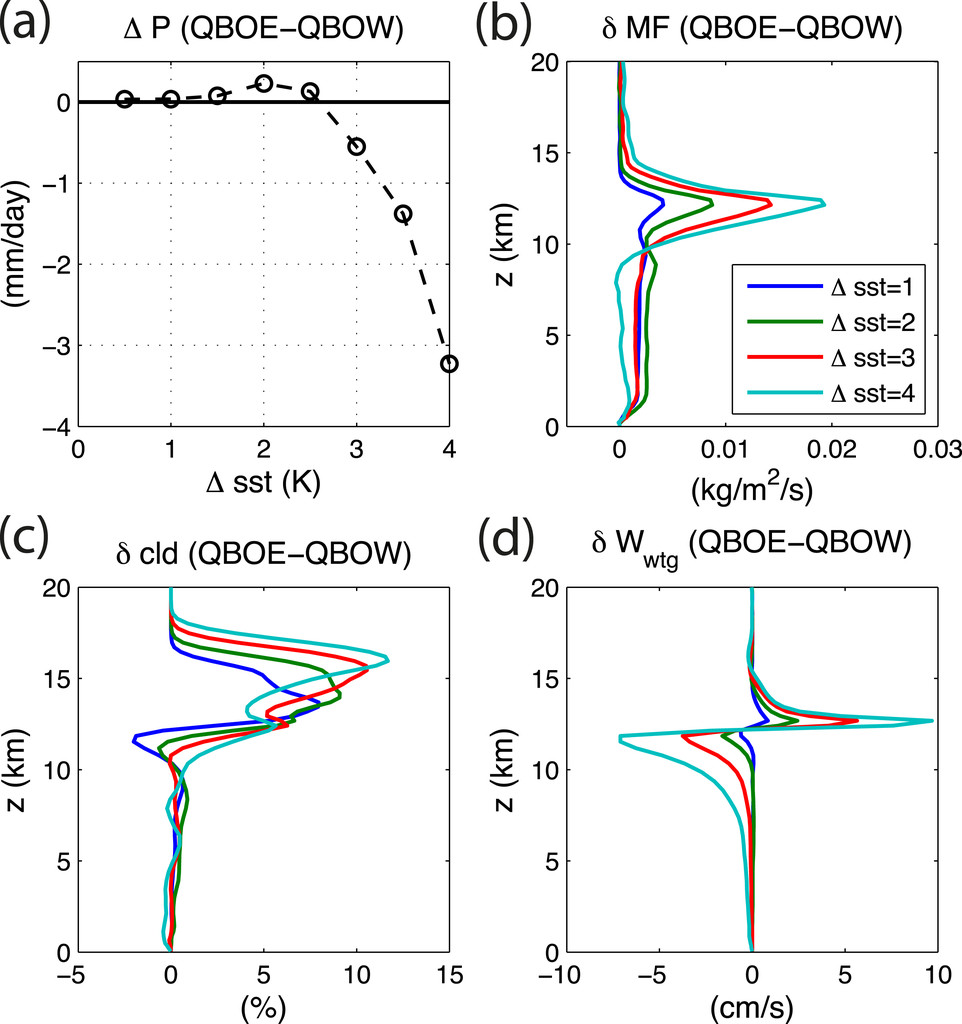
\includegraphics[width=0.85\linewidth]{figures/nie_sobel}
\caption[The non-linear relationship of the QBO with SST forcings]{(a) QBO anomalous precipitation as a function of SST forcing. The $\delta sst$ are increments over a baseline of 301 K throughout the whole model domain. (b)–(d) The differences of mass flux in cloud cores, cloud fraction, and the parametrized large-scale vertical velocity derived from the weak temperature gradient approximation, respectively, between experiments with the QBOE and QBOW temperature profiles. Figure 3 from \cite{nie2015}. }
\label{fig:nie}
\end{figure}  


\added{The suggestion that the variability in the UTLS static stability due to the QBO is arguably the leading hypothesis for the tropical route of QBO teleconnections \citep{giorgetta1999,liess2012,nie2015}. In short, this argument suggests that a upper-level static stability, decreased under QBOE and increased under QBOW, can impact the strength of convection. }
 The response of convection to the UTLS temperature anomalies associated with the QBO was investigated in cloud-resolving model simulations by \cite{nie2015}. Their experimental design varied SST boundary conditions with increments over a baseline SST level of 301 K,  using the weak-temperature gradient (WTG) \footnote{The weak temperature gradient approximation makes use of the relatively small horizontal gradients of temperature and density in the tropics, which simplifies some of the primitive equations and has allowed several numerical analyses of tropical dynamics using simplified models \citep{sobel2001wtg}.} approximation and an idealized vertical temperature profile to simulate the effect of the QBO temperature signal. 
 
 Figure \ref{fig:nie} shows that the precipitation differences between QBO phases depend on the SST forcing.   The precipitation difference between QBO temperature anomalies is positive under relatively small SST anomalies but in experiments with large SST anomalies this difference becomes negative and overall larger than under small SSTs. The difference in mass flux and cloud fraction is also sensitive to the underlying SSTs, as increased mass flux during QBOE is increased for larger SSTs.  In other words, the QBO influence on precipitation is non monotonic and largely depends on the underlying SST field.
 
%  The cloud fraction in the upper troposphere is increased during QBOE compared to QBOW whereas the ascending motions show peculiar behaviour with stronger ascent above 12 km for QBOE and weaker ascent below 12 km. 
  The results of \cite{nie2015} suggest that the QBO influences convection in two ways that are non-linear and that are the result of competing mechanisms. Their argument is that since  the mass flux in the upper troposphere is increased during QBOE but there is also an increase in gross moist static stability (GMS) the result is an increase in the efficiency of large-scale vertical motions during QBOE for large SSTs, which acts to reduce precipitation.  Secondly, the QBO modifies the fraction of high-level clouds resulting from deep convection which modifies the radiative heating to the column which increases precipitation during QBOE.  Figure \ref{fig:nie}a then shows how these competing effects change for different SSTs with the gross moist stability mechanism dominating for large SSTs.



One influential study by \cite{collimore2003} analysed satellite-derived out-going long-wave radiation (OLR) in the tropics composited by QBO phase. These composites suggest that OLR is significantly different between QBO phases in most monsoon regions, such as Central America  and the West Pacific, with an overall indication that convective activity is reduced during QBOW compared to QBOE. This influence, however, was not found to be zonally symmetric and in fact the longitudinal variations of the QBO-related OLR differences were suggestive enough that \cite{collimore2003} argue for a possible role for the QBO to modulate the Walker circulation, which would explain the lack of zonal symmetry in their results. 

Further modelling work has been carried out, for instance by \cite{garfinkel2010} and \cite{garfinkel2011} that investigate the effect of the QBO over tropical precipitation, the subtropical jets and the wintertime polar vortex in a GCM. \cite{garfinkel2010} shows that the canonical ENSO teleconnections to the North Pacific are stronger during QBOW suggesting that the QBO modulates the wave propagation activity associated with ENSO events.
 \cite{garfinkel2011} uses perpetual winter conditions in the GCM to show that the QBO modifies the upper-tropospheric zonal wind at the equator and the strength and location of subtropical jets, as the subtropical jet is weakened during QBOE conditions.


Another relevant study by \cite{liess2012} found that satellite-derived cloud thickness and frequency  and upper-level velocity potential had a significant and longitudinally asymmetric response to the QBO. In particular, their results show increased convective activity during QBOE in the West Pacific but the opposite for the East Pacific.  For this reason, \cite{liess2012} also argue that the strength of the tropical overturning circulation may be modulated by the QBO, indicating the possible role of both the vertical wind shear and the upper-level static stability to modulate deep convection. 
\added{\cite{liess2012} suggests the possibility of an indirect of the QBO, in which the QBO modulates the zonal tropical overturning circulation causing impacts of opposite signs at equatorial latitudes.}

The topic of QBO tropical teleconnections has regained attention due to recent findings suggesting a link between the QBO and the MJO \citep{son2017} which motivated extensive research \citep[see e.g.][]{lee2018,wang2019,martin2020jgr} due to the worldwide impact of the MJO.
 The MJO in observations shows a stronger amplitude and more predictability during QBOE, but further inspection in cloud-permitting and forecast models have not provided conclusive answers to this puzzle \citep{martin2019,martin2020jgr}. 
 
 \added{In short, multiple lines of evidence suggest relationships between the QBO and tropical convection.  The leading hypothesis for these relationships suggests that the modulation of the UTLS temperature structure influences the upper-level static stability to the extent that the QBO can influence the strength of ascent. The effect of the QBO on vertical shear and feebacks with the tropical overturning circulation have also been suggested as possible explanations for the observed responses to the QBO phase.  }
 
 \added{Questions still arise as to whether this tropical link is real or due to chance, for instance \cite{wang2019} argued that the increased predictability of the MJO under the QBOE phase is included in the initial conditions, and thus not a result of a mechanistic effect of the QBO on the MJO. More generally, whether the QBO has a considerable effect on deep convection in general is debated as several plausible mechanisms exist in the literature \citep[see e.g.][]{nie2015} such as the effect of wind shear, the tropopause height, the cold-point temperature, static stability and/or feedbacks with very high cirrus and cumulunimbus clouds or the tropical circulation. }
%The use of climate models to understand these tropical teleconnections of the QBO has proven difficult due to biases in both the MJO and the QBO representations. State-of-the-art CMIP6 models struggle to reproduce several of the characteristics of the QBO \citep{richter2020}. For instance,  weaker temperature QBO signals in the lowermost tropical stratosphere in the models, e.g., compare the QBOE-W difference plot in Figure \ref{fig:qbo}. The weaker temperature signal may be key for possible biases in the tropical QBO links discussed above, such as the the QBO-MJO link which is missing from CMIP6 models \citep{kim2020} and from seasonal prediction forecast models \citep{wang2019,martin2020jgr}. 